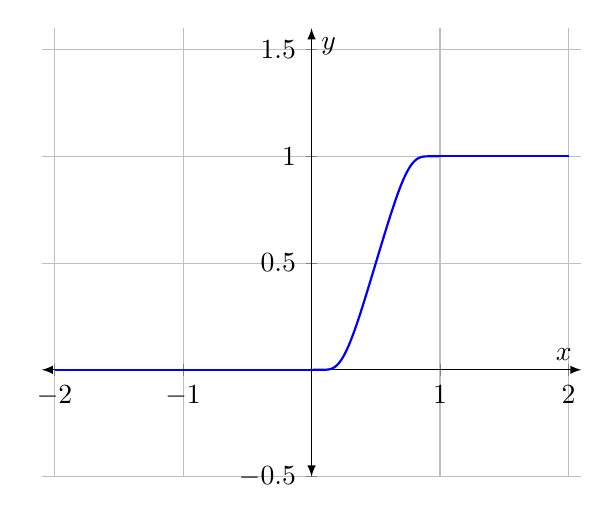
\begin{tikzpicture}
\begin{axis}[
  grid=both,
  xmin=-2.1,
  xmax=2.1,
  ymin=-0.5,
  ymax=1.6,
  axis lines=middle,
  xlabel = $x$,
  ylabel = $y$,
  axis line style={latex-latex},
  ]

\addplot[
  samples=100,
  domain=0.01:0.99,
  color=blue,
  thick,
  smooth,
  ]
  {((e)^(-1/x)) / ( ( e^(-1/x) ) + (e^(-1/(1-x))) )};


\addplot[
  samples=2,
  domain=-2:0.01,
  color=blue,
  thick,
  smooth
  ]
  {0};

\addplot[
  samples=2,
  domain=0.99:2,
  color=blue,
  thick,
  smooth
  ]
  {1};
\end{axis}
\end{tikzpicture}
